\documentclass{book}
\usepackage[british]{babel}
\usepackage{tikz-feynman}

\begin{document}
 
\feynmandiagram [horizontal=a to b] {
	i1 [particle=\(b\)] -- [fermion] a -- [fermion] i2 [particle=\(\overline b\)],
	a -- [photon, edge label=\(\gamma/Z^{0}\)] b,
	f1 [particle=\(\ell^{+}\)] -- [fermion] b -- [fermion] f2 [particle=\(\ell^{-}\)],
};

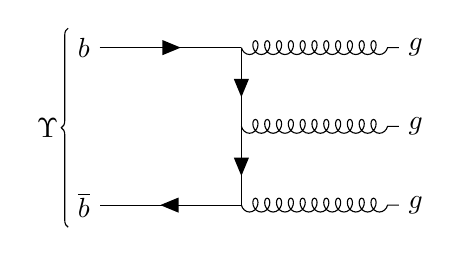
\begin{tikzpicture}
  \begin{feynman}
    \vertex (a1) {\(b\)};
    \vertex[right=2cm of a1] (a2);
    \vertex[below=1cm of a2] (a3);
    \vertex[below=1cm of a3] (a4);
    \vertex[left=1.8cm of a4] (a5){\(\overline b\)};

    \vertex[right=0cm of a2] (b1);
    \vertex[right=2cm of b1] (b2) {\(g\)};
    
    \vertex[right=0cm of a3] (c1);
    \vertex[right=2cm of c1] (c2) {\(g\)};
    
    \vertex[right=0cm of a4] (d1);
    \vertex[right=2cm of d1] (d2) {\(g\)};

    \diagram* {
      {[edges=fermion]
        (a1) -- (a2) -- (a3) -- (a4) -- (a5),
      },
      (b1) -- [gluon] (b2),
      (c1) -- [gluon] (c2),
      (d1) -- [gluon] (d2),
    };

    \draw [decoration={brace}, decorate] (a5.south west) -- (a1.north west)
          node [pos=0.5, left] {\(\Upsilon\)};
  \end{feynman}
\end{tikzpicture}

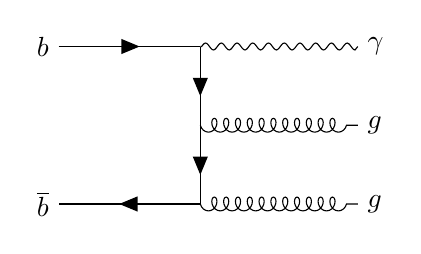
\begin{tikzpicture}
  \begin{feynman}
    \vertex (a1) {\(b\)};
    \vertex[right=2cm of a1] (a2);
    \vertex[below=1cm of a2] (a3);
    \vertex[below=1cm of a3] (a4);
    \vertex[left=1.8cm of a4] (a5){\(\overline b\)};

    \vertex[right=0cm of a2] (b1);
    \vertex[right=2cm of b1] (b2) {\(\gamma\)};
    
    \vertex[right=0cm of a3] (c1);
    \vertex[right=2cm of c1] (c2) {\(g\)};
    
    \vertex[right=0cm of a4] (d1);
    \vertex[right=2cm of d1] (d2) {\(g\)};

    \diagram* {
      {[edges=fermion]
        (a1) -- (a2) -- (a3) -- (a4) -- (a5),
      },
      (b1) -- [photon] (b2),
      (c1) -- [gluon] (c2),
      (d1) -- [gluon] (d2),
    };

  \end{feynman}
\end{tikzpicture}\\
% \feynmandiagram [horizontal=a to b] {
% 	a [particle=\(\mu^{-}\)] -- [fermion] b -- [fermion] f1 [particle=\(\nu_{\mu}\)],
% 	b -- [boson, edge label=\(W^{-}\)] c,
% 	f2 [particle=\(\overline \nu_{e}\)] -- [fermion] c -- [fermion] f3 [particle=\(e^{-}\)],
% };
\feynmandiagram [layered layout, horizontal=a to b] {
a [particle=\(t\)] -- [fermion] b -- [fermion] f1 [particle=\(b\)],
b -- [boson, edge label'=\(W^{+}\)] c,
c -- [anti fermion] f2 [particle=\(\ell^+\)],
c -- [fermion] f3 [particle=\(\nu\)],
};\\
\feynmandiagram [layered layout, horizontal=a to b] {
a [particle=\(t\)] -- [fermion] b -- [fermion] f1 [particle=\(b\)],
b -- [boson, edge label'=\(W^{+}\)] c,
c -- [anti fermion] f2 [particle=\(\overline{q}\)],
c -- [fermion] f3 [particle=\(q\)],
};\\
	
\feynmandiagram [horizontal=a to b] {
	i1 [particle=\(b\)] -- [fermion] a -- [fermion] i2 [particle=\(\overline u\)],
	a -- [boson, edge label=\(W^-\)] b,
	f1 [particle=\(\overline\nu/\overline{q}\)] -- [fermion] b -- [fermion] f2 [particle=\(\ell^{-}/q\)],
};\\
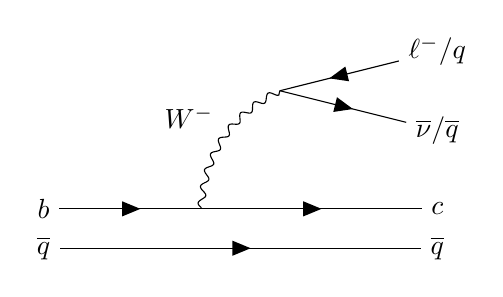
\begin{tikzpicture}
  \begin{feynman}
    \vertex (a1) {\(\overline q\)};
    \vertex[right=5cm of a1] (a2) {\(\overline q\)};
    
    \vertex[above=.5cm of a1] (b1) {\(b\)};
    \vertex[right=2cm of b1] (b2);
    \vertex[right=2.8cm of b2] (b3) {\(c\)};
    
    \vertex[above=1cm of b3] (c1) {\(\overline\nu/\overline{q}\)};
    \vertex[above=1cm of c1] (c3) {\(\ell^{-}/q\)};
    \vertex at ($(c1)!0.5!(c3) - (2cm, 0)$) (c2);

    \diagram* {
      {[edges=fermion] (b1) -- (b2) -- (b3)},
      {[edges=fermion] (c3) -- (c2) -- (c1)},
      (a1) -- [fermion] (a2),
      (b2) -- [boson, bend left, edge label=\(W^{-}\)] (c2),
    };

  \end{feynman}
\end{tikzpicture}\\
	
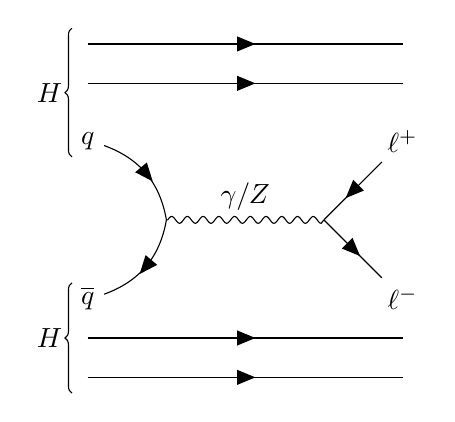
\begin{tikzpicture}
  \begin{feynman}
    \vertex (a1);
    \vertex[right=4cm of a1] (a2);
    
    \vertex[below=.5cm of a1] (b1);
    \vertex[right=4cm of b1] (b2);
    
    \vertex[below=.5cm of b1] (c1) {\(q\)};
    \vertex[below=2cm of c1] (c3) {\(\overline q\)};
    \vertex at ($(c1)!0.5!(c3) + (1cm, 0)$) (c2);
    
    \vertex[right=2cm of c2] (f1);
    \vertex[right=4cm of c1] (f2) {\(\ell^{+}\)};
    \vertex[right=4cm of c3] (f3) {\(\ell^{-}\)};
    
    \vertex[below=.5cm of c3] (d1);
    \vertex[right=4cm of d1] (d2);
    
    \vertex[below=.5cm of d1] (e1);
    \vertex[right=4cm of e1] (e2);
    
    \diagram* {
      (c1) -- [fermion, bend left] (c2),
      (c2) -- [fermion, bend left] (c3),
      (a1) -- [fermion] (a2),
      (b1) -- [fermion] (b2),
      (d1) -- [fermion] (d2),
      (e1) -- [fermion] (e2),
      (c2) -- [boson, edge label=\(\gamma/Z\)] (f1),
      {[edges=fermion] (f2) -- (f1) -- (f3)},
    };
    \draw [decoration={brace}, decorate] ($(c1) - (.2cm,.2cm)$) -- ($(a1) + (-.2cm,0.2cm)$)
          node [pos=0.5, left] {\(H\)};
    \draw [decoration={brace}, decorate] ($(e1) - (.2cm,.2cm)$) -- ($(c3) + (-.2cm,0.2cm)$)
          node [pos=0.5, left] {\(H\)};

  \end{feynman}
\end{tikzpicture}\\
\end{document}
